% Options for packages loaded elsewhere
\PassOptionsToPackage{unicode}{hyperref}
\PassOptionsToPackage{hyphens}{url}
%
\documentclass[
  letterpaper,
  ignorenonframetext,
  aspectratio=43,
  handout,
  12pt]{beamer}
\usepackage{pgfpages}
\setbeamertemplate{caption}[numbered]
\setbeamertemplate{caption label separator}{: }
\setbeamercolor{caption name}{fg=normal text.fg}
\beamertemplatenavigationsymbolsempty
% Prevent slide breaks in the middle of a paragraph
\widowpenalties 1 10000
\raggedbottom
\setbeamertemplate{part page}{
  \centering
  \begin{beamercolorbox}[sep=16pt,center]{part title}
    \usebeamerfont{part title}\insertpart\par
  \end{beamercolorbox}
}
\setbeamertemplate{section page}{
  \centering
  \begin{beamercolorbox}[sep=12pt,center]{part title}
    \usebeamerfont{section title}\insertsection\par
  \end{beamercolorbox}
}
\setbeamertemplate{subsection page}{
  \centering
  \begin{beamercolorbox}[sep=8pt,center]{part title}
    \usebeamerfont{subsection title}\insertsubsection\par
  \end{beamercolorbox}
}
\AtBeginPart{
  \frame{\partpage}
}
\AtBeginSection{
  \ifbibliography
  \else
    \frame{\sectionpage}
  \fi
}
\AtBeginSubsection{
  \frame{\subsectionpage}
}
\usepackage{amsmath,amssymb}
\usepackage{lmodern}
\usepackage{ifxetex,ifluatex}
\ifnum 0\ifxetex 1\fi\ifluatex 1\fi=0 % if pdftex
  \usepackage[T1]{fontenc}
  \usepackage[utf8]{inputenc}
  \usepackage{textcomp} % provide euro and other symbols
\else % if luatex or xetex
  \usepackage{unicode-math}
  \defaultfontfeatures{Scale=MatchLowercase}
  \defaultfontfeatures[\rmfamily]{Ligatures=TeX,Scale=1}
\fi
\usetheme[]{metropolis}
% Use upquote if available, for straight quotes in verbatim environments
\IfFileExists{upquote.sty}{\usepackage{upquote}}{}
\IfFileExists{microtype.sty}{% use microtype if available
  \usepackage[]{microtype}
  \UseMicrotypeSet[protrusion]{basicmath} % disable protrusion for tt fonts
}{}
\makeatletter
\@ifundefined{KOMAClassName}{% if non-KOMA class
  \IfFileExists{parskip.sty}{%
    \usepackage{parskip}
  }{% else
    \setlength{\parindent}{0pt}
    \setlength{\parskip}{6pt plus 2pt minus 1pt}}
}{% if KOMA class
  \KOMAoptions{parskip=half}}
\makeatother
\usepackage{xcolor}
\IfFileExists{xurl.sty}{\usepackage{xurl}}{} % add URL line breaks if available
\IfFileExists{bookmark.sty}{\usepackage{bookmark}}{\usepackage{hyperref}}
\hypersetup{
  hidelinks,
  pdfcreator={LaTeX via pandoc}}
\urlstyle{same} % disable monospaced font for URLs
\newif\ifbibliography
\usepackage{graphicx}
\makeatletter
\def\maxwidth{\ifdim\Gin@nat@width>\linewidth\linewidth\else\Gin@nat@width\fi}
\def\maxheight{\ifdim\Gin@nat@height>\textheight\textheight\else\Gin@nat@height\fi}
\makeatother
% Scale images if necessary, so that they will not overflow the page
% margins by default, and it is still possible to overwrite the defaults
% using explicit options in \includegraphics[width, height, ...]{}
\setkeys{Gin}{width=\maxwidth,height=\maxheight,keepaspectratio}
% Set default figure placement to htbp
\makeatletter
\def\fps@figure{htbp}
\makeatother
% Make links footnotes instead of hotlinks:
\DeclareRobustCommand{\href}[2]{#2\footnote{\url{#1}}}
\setlength{\emergencystretch}{3em} % prevent overfull lines
\providecommand{\tightlist}{%
  \setlength{\itemsep}{0pt}\setlength{\parskip}{0pt}}
\setcounter{secnumdepth}{-\maxdimen} % remove section numbering
\usepackage{pgfpages}
\pgfpagesuselayout{2 on 1}
\providecommand{\tightlist}{%
\setlength{\itemsep}{0pt}\setlength{\parskip}{0pt}}
\makeatletter
\makeatother
\let\Oldincludegraphics\includegraphics
\renewcommand{\includegraphics}[2][]{\Oldincludegraphics[width=\textwidth,height=0.7\textheight,keepaspectratio]{#2}}
\ifluatex
  \usepackage{selnolig}  % disable illegal ligatures
\fi

\author{}
\date{}

\begin{document}

\begin{frame}{AE 737: Mechanics of Damage Tolerance}
\protect\hypertarget{ae-737-mechanics-of-damage-tolerance}{}
Lecture 13 - Project Discussion

Dr.~Nicholas Smith

Wichita State University, Department of Aerospace Engineering

March 17, 2021
\end{frame}

\begin{frame}{schedule}
\protect\hypertarget{schedule}{}
\begin{itemize}
\tightlist
\item
  17 Mar - Project Discussion, Fatigue
\item
  19 Mar - HW5 Self-grade due
\item
  22 Mar - Stress-based Fatigue
\item
  24 Mar - Stress-based Fatigue
\item
  26 Mar - Project Abstract Due
\item
  29 Mar - Strain-based Fatigue
\end{itemize}
\end{frame}

\begin{frame}{outline}
\protect\hypertarget{outline}{}
\begin{itemize}
\tightlist
\item
  exam
\item
  final project
\item
  fatigue
\item
  nominal and local stress
\item
  fatigue tests
\end{itemize}
\end{frame}

\hypertarget{exam}{%
\section{exam}\label{exam}}

\begin{frame}{curve}
\protect\hypertarget{curve}{}
\end{frame}

\hypertarget{final-project}{%
\section{final project}\label{final-project}}

\begin{frame}{general description}
\protect\hypertarget{general-description}{}
\begin{itemize}
\tightlist
\item
  This is in place of a final exam
\item
  Should demonstrate your understanding of the course as a whole
\item
  Choose any real object
\item
  Needs to undergo some cyclic loading (for fatigue)
\item
  Materials, loads, and any other ``given'' data can be made up
\end{itemize}
\end{frame}

\begin{frame}{overview}
\protect\hypertarget{overview}{}
\begin{itemize}
\tightlist
\item
  Estimate stress intensity factor at some critical location
\item
  Estimate residual strength (use a ``typical'' crack length)
\item
  Estimate fatigue life
\item
  Estimate crack propagation
\item
  Suggest reasonable inspection cycle for safe use
\item
  Suggest an improvement to make part more damage tolerant
\end{itemize}
\end{frame}

\begin{frame}{grade breakdown}
\protect\hypertarget{grade-breakdown}{}
\begin{itemize}
\tightlist
\item
  Per course syllabus, project will be worth 25\% of final grade
\item
  5\% Project abstract submission and approval
\item
  15\% for each major component

  \begin{itemize}
  \tightlist
  \item
    stress intensity factor
  \item
    residual strength
  \item
    fatigue
  \item
    crack propagation
  \item
    inspection cycle
  \end{itemize}
\end{itemize}
\end{frame}

\begin{frame}{grade breakdown}
\protect\hypertarget{grade-breakdown-1}{}
\begin{itemize}
\tightlist
\item
  10\% for damage tolerant improvement
\item
  10\% general presentation, organization, and grammar
\end{itemize}
\end{frame}

\begin{frame}{project abstract}
\protect\hypertarget{project-abstract}{}
\begin{itemize}
\tightlist
\item
  Main purpose of abstract is for you to make sure your idea fits with
  project purpose
\item
  I will give you feedback on how to tweak your proposed idea to better
  meet project purpose
\item
  Abstract submission should be 1-2 pages
\item
  Briefly describe your chosen part, how it undergoes cyclic loading,
  what location you intend to consider for the stress intensity factor.
\item
  This is like a proposal: convince me that your idea has what it takes
  to be a great final project
\end{itemize}
\end{frame}

\begin{frame}{justify assumptions}
\protect\hypertarget{justify-assumptions}{}
\begin{itemize}
\tightlist
\item
  You will need to make many assumptions in order to complete this
  project
\item
  Clearly state your assumptions and justify them (i.e.~if you assume
  plane strain conditions, justify that by showing how thick your part
  is)
\item
  Although will not have experimental or FE analysis specific to your
  part, use concepts from other data in the text (stiffeners, multiple
  site damage) in a qualitative manner
\end{itemize}
\end{frame}

\begin{frame}{figures}
\protect\hypertarget{figures}{}
\begin{itemize}
\tightlist
\item
  Figures can greatly enhance your project report, if you use them well
\item
  Many readers will jump to figures in a report, include sufficient
  information in caption and axis labels so a reader with general damage
  tolerance understanding can understand your figure
\item
  This will interest them in the rest of your paper
\end{itemize}
\end{frame}

\begin{frame}{examples}
\protect\hypertarget{examples}{}
\begin{itemize}
\tightlist
\item
  Last year I did not curve final project grades
\item
  Some examples of a couple of good project reports have been posted to
  blackboard (and
  \href{https://ndaman.github.io/damagetolerance/\#/2/2}{here})
\item
  You should not use their projects, but they have very good use of
  figures, as well as an appropriate balance of both depth and breadth
  in the their analysis
\end{itemize}
\end{frame}

\hypertarget{fatigue}{%
\section{fatigue}\label{fatigue}}

\begin{frame}{fatigue}
\protect\hypertarget{fatigue-1}{}
\begin{itemize}
\tightlist
\item
  We refer to damage from repeated, or cyclic loads as fatigue damage
\item
  Some of the earliest work on fatigue began in the 1800's
\item
  Chains, railway axles, etc.
\item
  An estimated 80\% of failure expenses are due to fatigue
\end{itemize}
\end{frame}

\begin{frame}{fatigue}
\protect\hypertarget{fatigue-2}{}
\begin{itemize}
\tightlist
\item
  There are three main approaches to fatigue analysis

  \begin{itemize}
  \tightlist
  \item
    Stress based fatigue analysis
  \item
    Strain based fatigue analysis
  \item
    Fracture mechanics fatigue analysis
  \end{itemize}
\end{itemize}
\end{frame}

\begin{frame}{stress based fatigue}
\protect\hypertarget{stress-based-fatigue}{}
\begin{itemize}
\tightlist
\item
  One of the simplest assumptions we can make is that a load cycles
  between a constant maximum and minimum stress value
\item
  This is a good approximation for many cases (axles, for example) and
  can also be easily replicated experimentally
\item
  This is referred to as constant amplitude stressing
\end{itemize}
\end{frame}

\begin{frame}{constant amplitude stressing}
\protect\hypertarget{constant-amplitude-stressing}{}
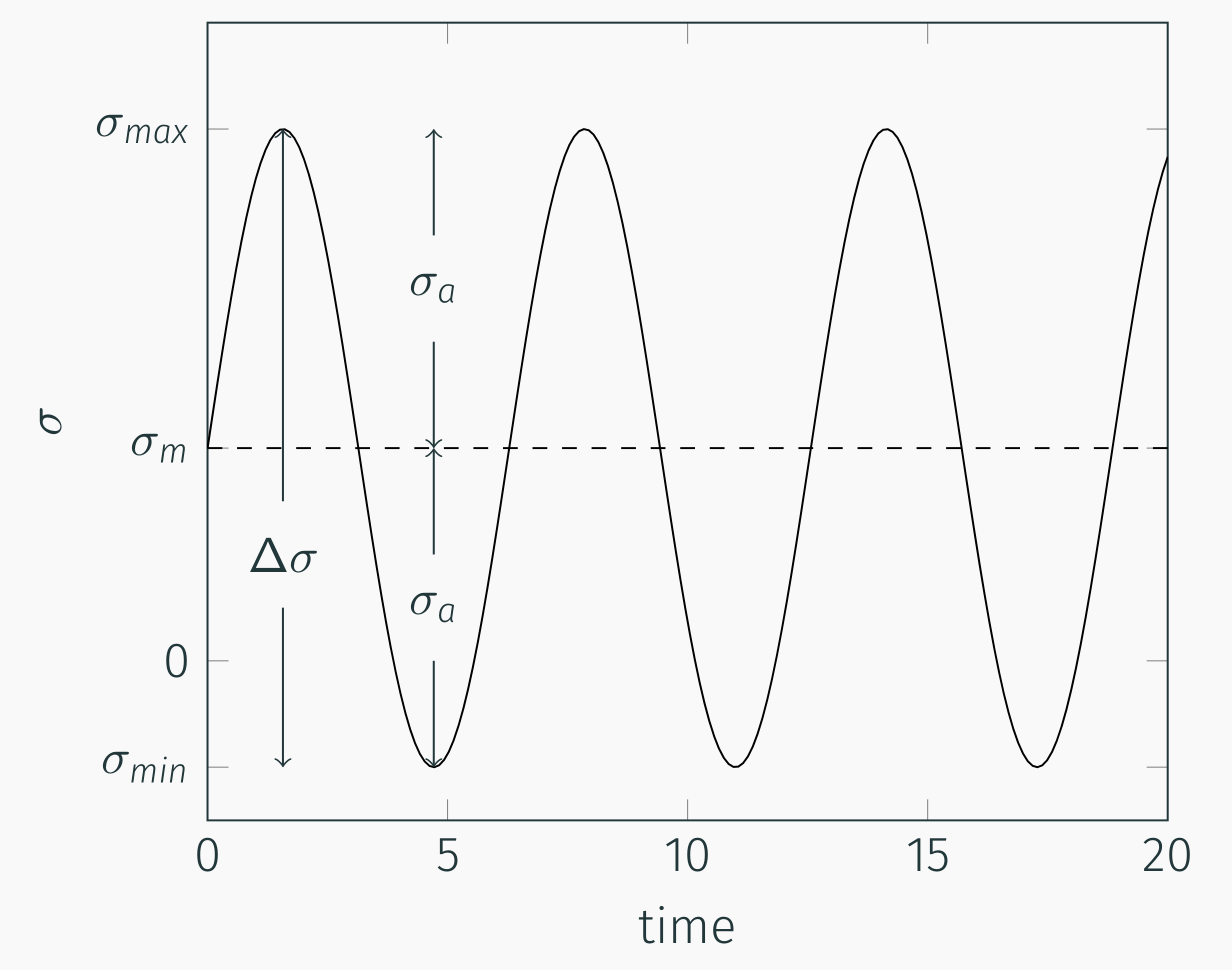
\includegraphics{../images/fatigue-constant-amplitude.PNG}
\end{frame}

\begin{frame}{constant amplitude stressing}
\protect\hypertarget{constant-amplitude-stressing-1}{}
\begin{itemize}
\tightlist
\item
  \(\Delta \sigma\) is known as the stress range, and is the difference
  between max and min stress
\item
  \(\sigma_m\) is the mean stress, and can sometimes be zero, but this
  is not always the case
\item
  \(\sigma_a\) is the stress amplitude, and is the variation about the
  mean
\end{itemize}
\end{frame}

\begin{frame}{constant amplitude stressing}
\protect\hypertarget{constant-amplitude-stressing-2}{}
\begin{itemize}
\tightlist
\item
  We can express all of these in terms of the maximum and minimum stress
\end{itemize}

\[\begin{aligned}
  \Delta \sigma &= \sigma_{max} - \sigma_{min}\\
  \sigma_m &= \frac{\sigma_{max} + \sigma_{min}}{2}\\
  \sigma_a &= \frac{\sigma_{max}- \sigma_{min}}{2}
\end{aligned}\]
\end{frame}

\begin{frame}{constant amplitude stressing}
\protect\hypertarget{constant-amplitude-stressing-3}{}
\begin{itemize}
\tightlist
\item
  It is also common to describe some ratios
\item
  The stress ratio, \emph{R} is defined as
\end{itemize}

\[R = \frac{\sigma_{min}}{\sigma_{max}}\]

\begin{itemize}
\tightlist
\item
  And the amplitude ratio, \emph{A} is defined as
\end{itemize}

\[A = \frac{\sigma_a}{\sigma_m}\]
\end{frame}

\begin{frame}{useful relations}
\protect\hypertarget{useful-relations}{}
\begin{itemize}
\tightlist
\item
  There are some useful relationships between the above equations
\end{itemize}

\[\begin{aligned}
  \Delta \sigma &= 2 \sigma_a = \sigma_{max}(1-R)\\
  \sigma_m &= \frac{\sigma_{max}}{2}(1+R)\\
  R &= \frac{1-A}{1+A}\\
  A &= \frac{1-R}{1+R}
\end{aligned}\]
\end{frame}

\hypertarget{nominal-and-local-stress}{%
\section{nominal and local stress}\label{nominal-and-local-stress}}

\begin{frame}{definition and notation}
\protect\hypertarget{definition-and-notation}{}
\begin{itemize}
\tightlist
\item
  It is important to distinguish between the nominal (global) stress and
  the local stress at some point of interest
\item
  We use \(\sigma\) for the stress at a point (local stress)
\item
  We use \emph{S} as the nominal (global) stress
\item
  In simple tension, \$\sigma=S\$
\end{itemize}
\end{frame}

\begin{frame}{notation}
\protect\hypertarget{notation}{}
\begin{itemize}
\tightlist
\item
  For many cases (bending, notches), \(\sigma \ne S\) in general
\item
  We must also be careful to note \(\sigma_y\), in some cases
  \(S < \sigma_y\) but at some locations \(\sigma > \sigma_y\)
\end{itemize}
\end{frame}

\begin{frame}{simple tension}
\protect\hypertarget{simple-tension}{}
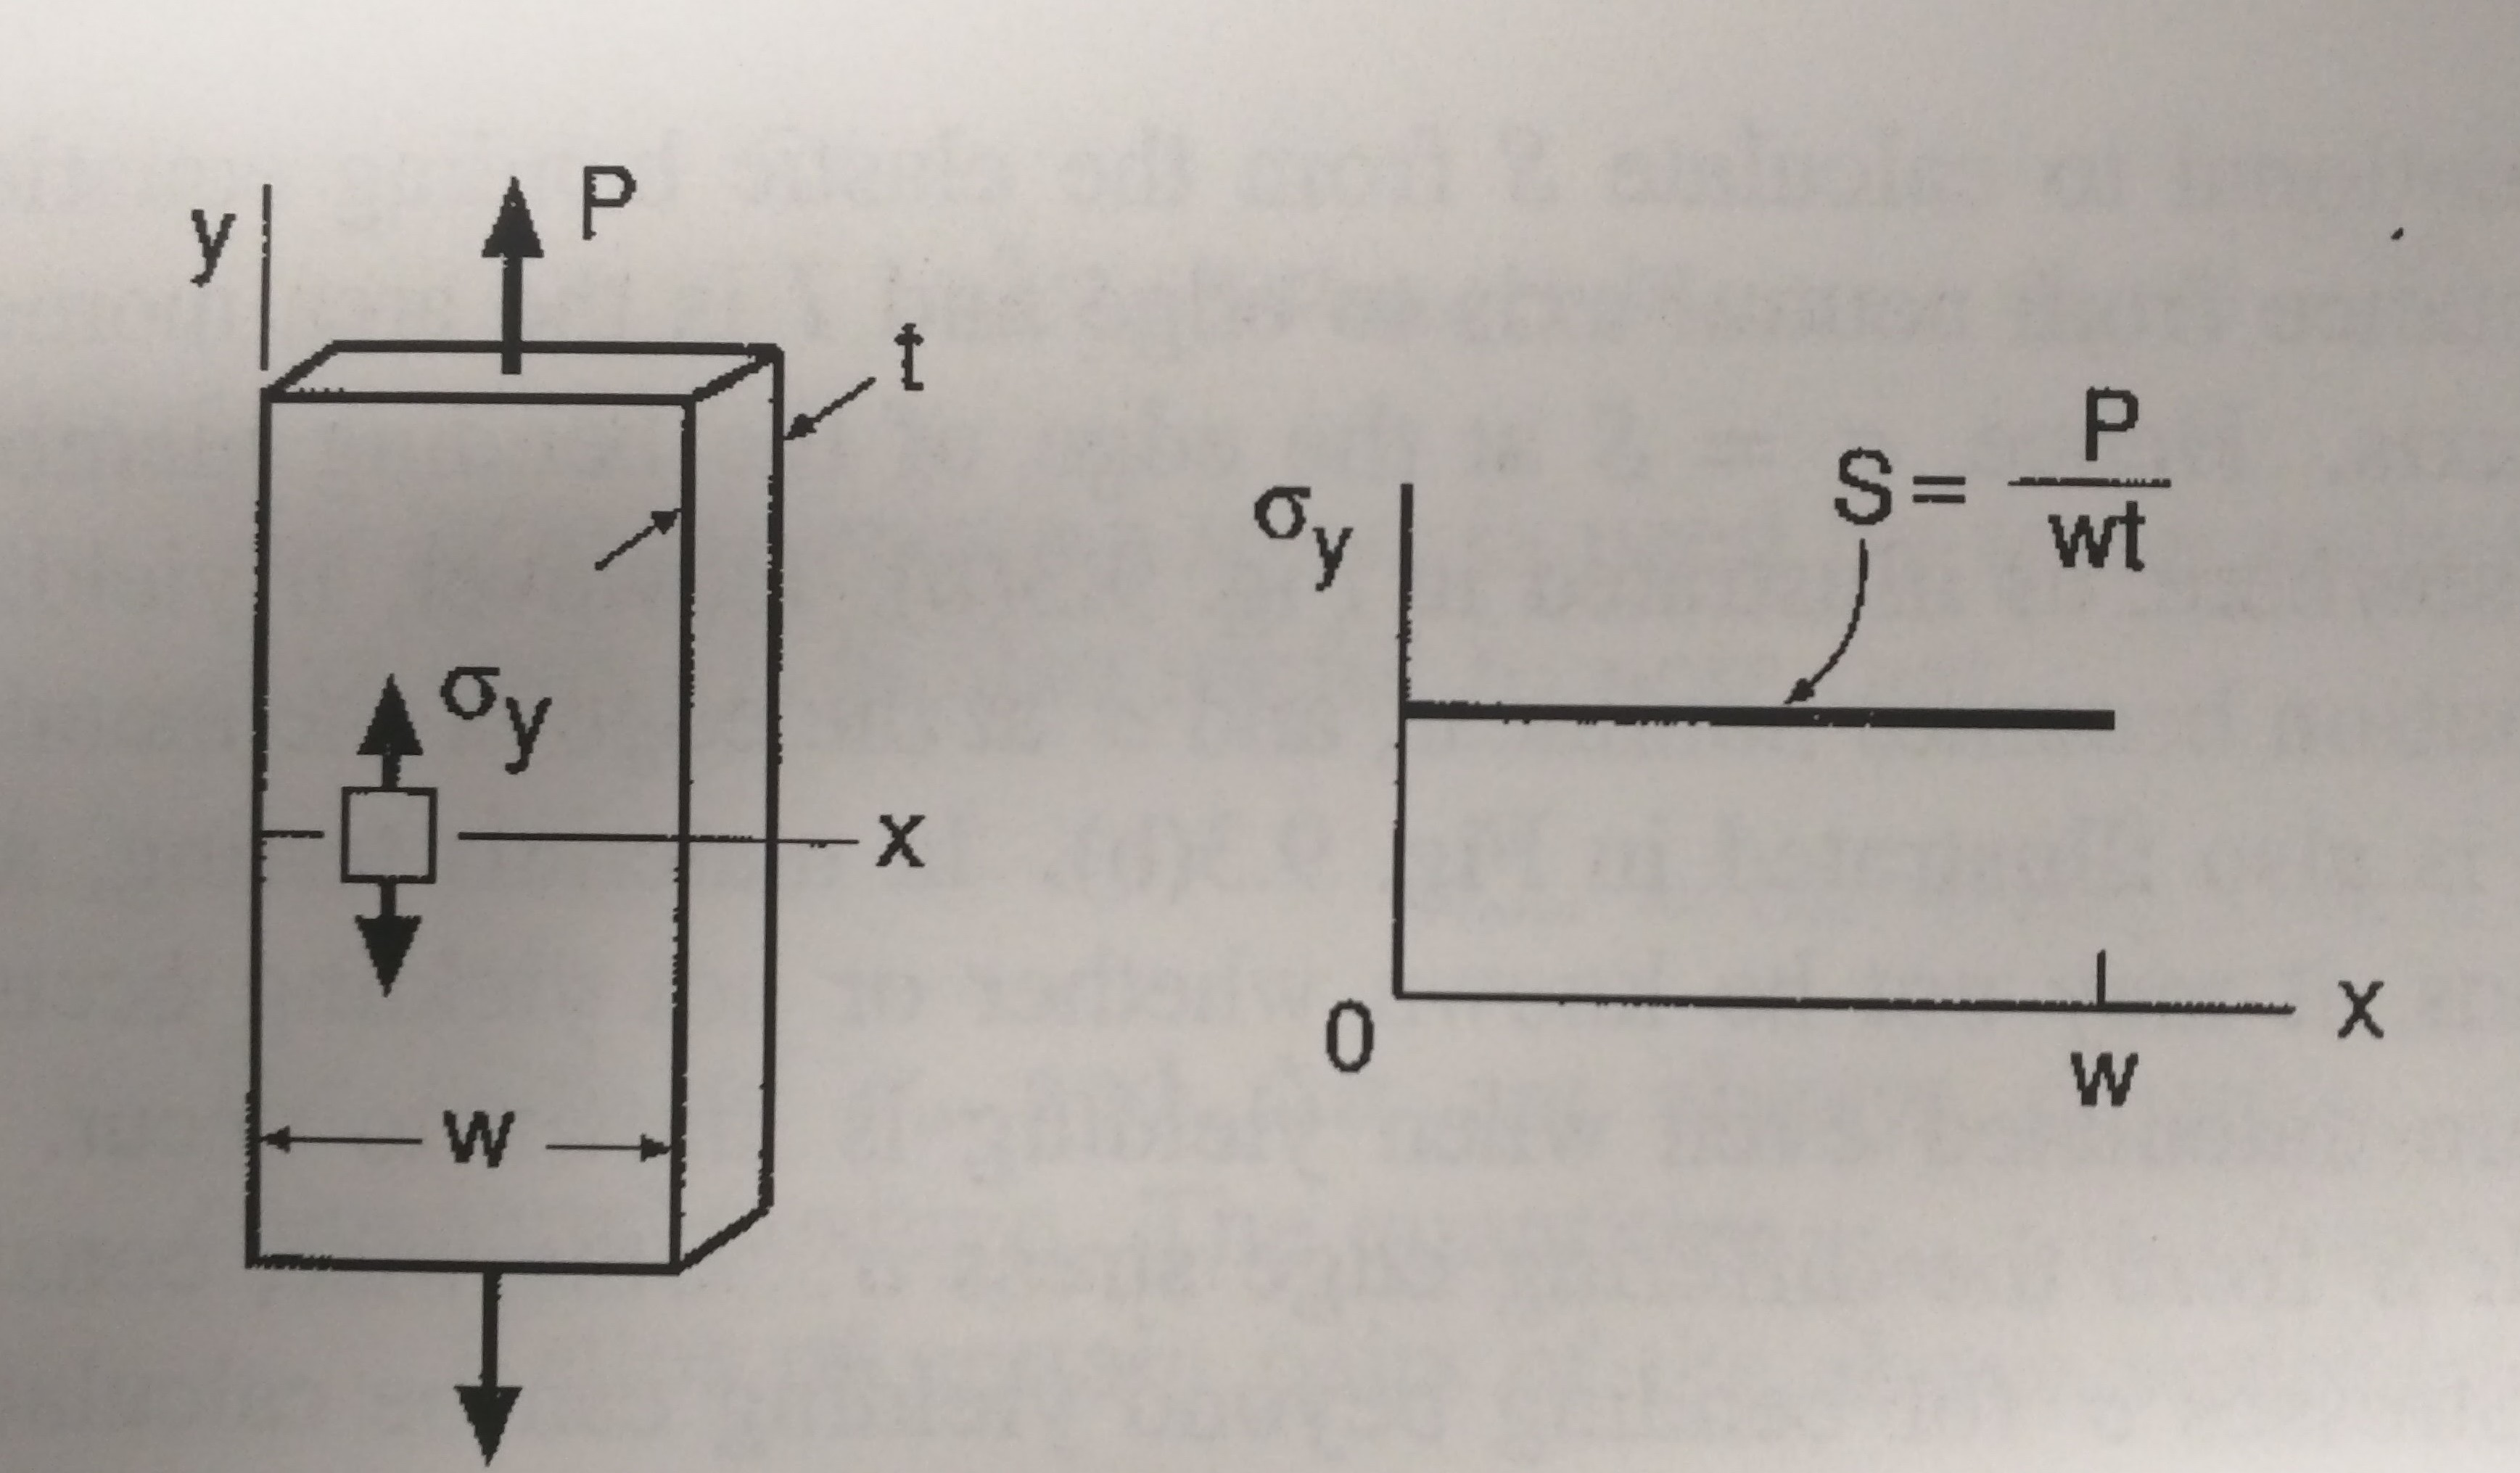
\includegraphics{../images/p232-a.jpg}
\end{frame}

\begin{frame}{bending}
\protect\hypertarget{bending}{}
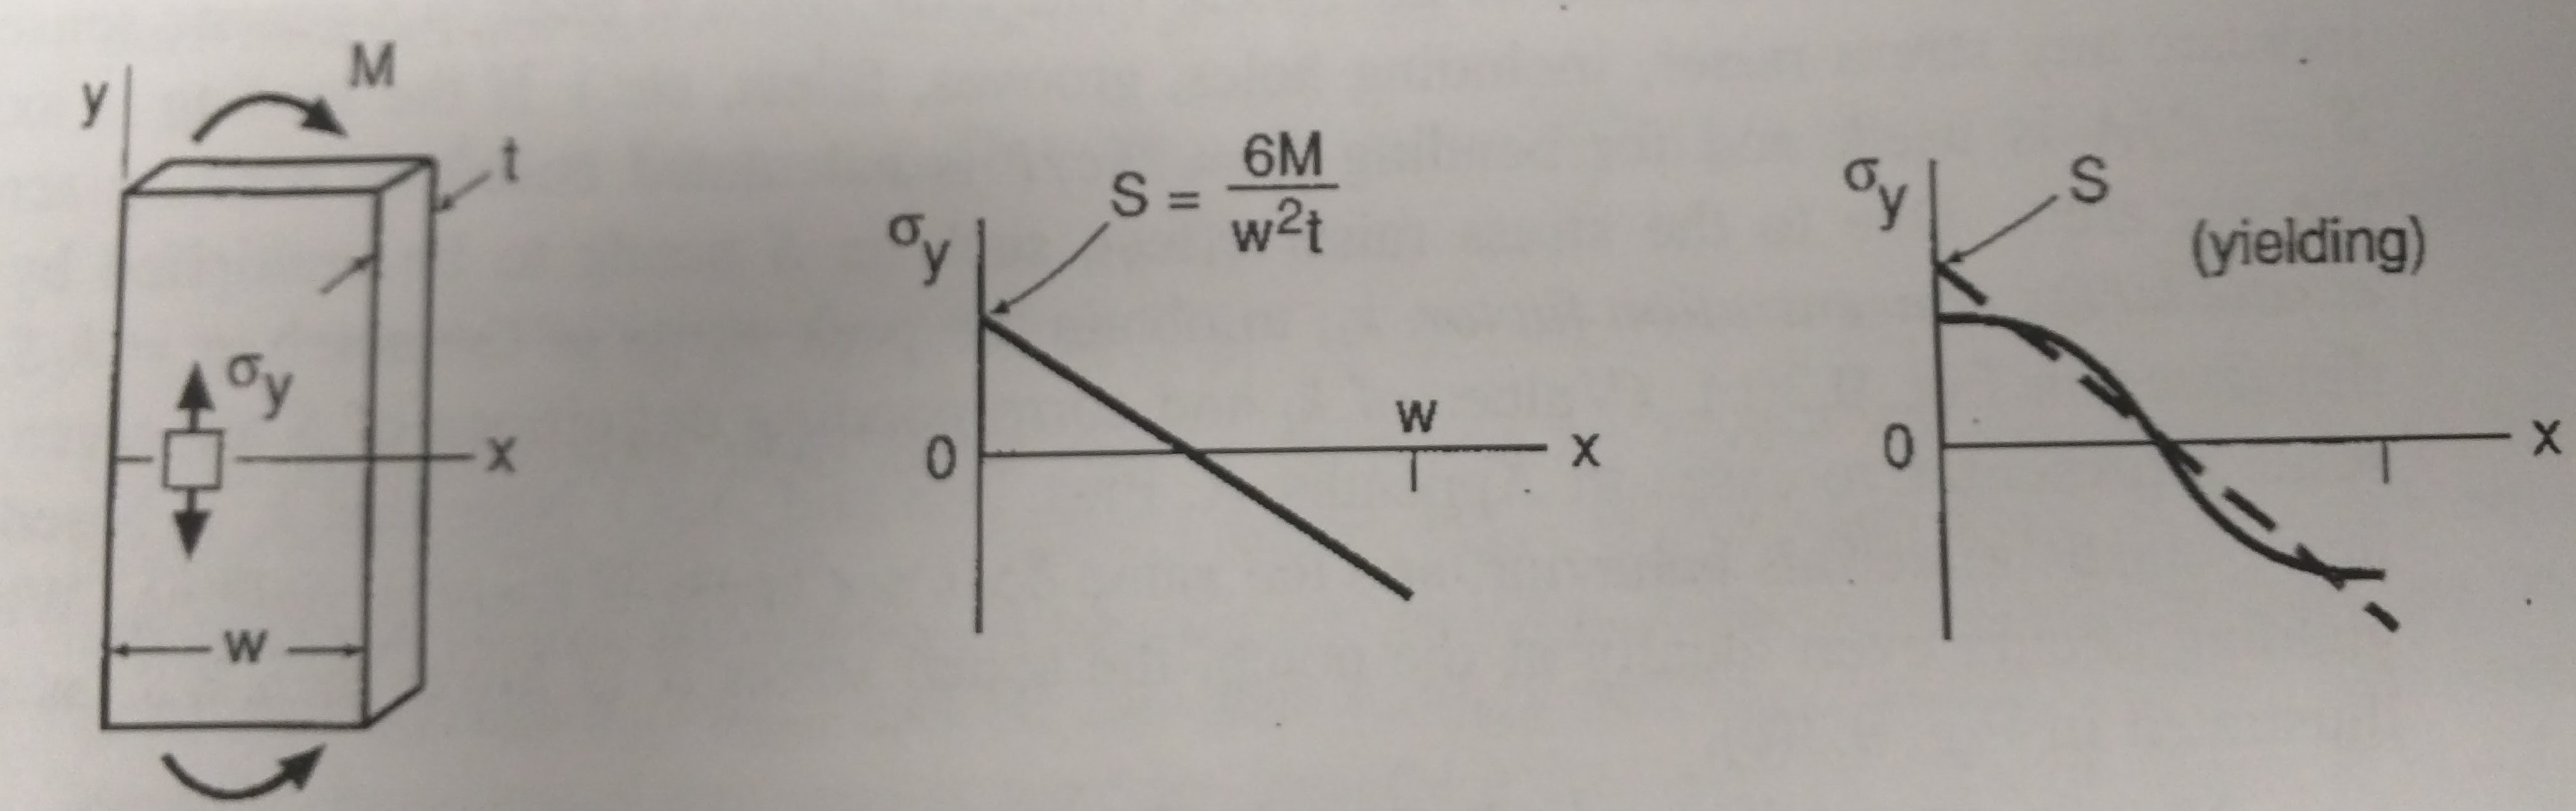
\includegraphics{../images/p232-b.jpg}
\end{frame}

\begin{frame}{notches}
\protect\hypertarget{notches}{}
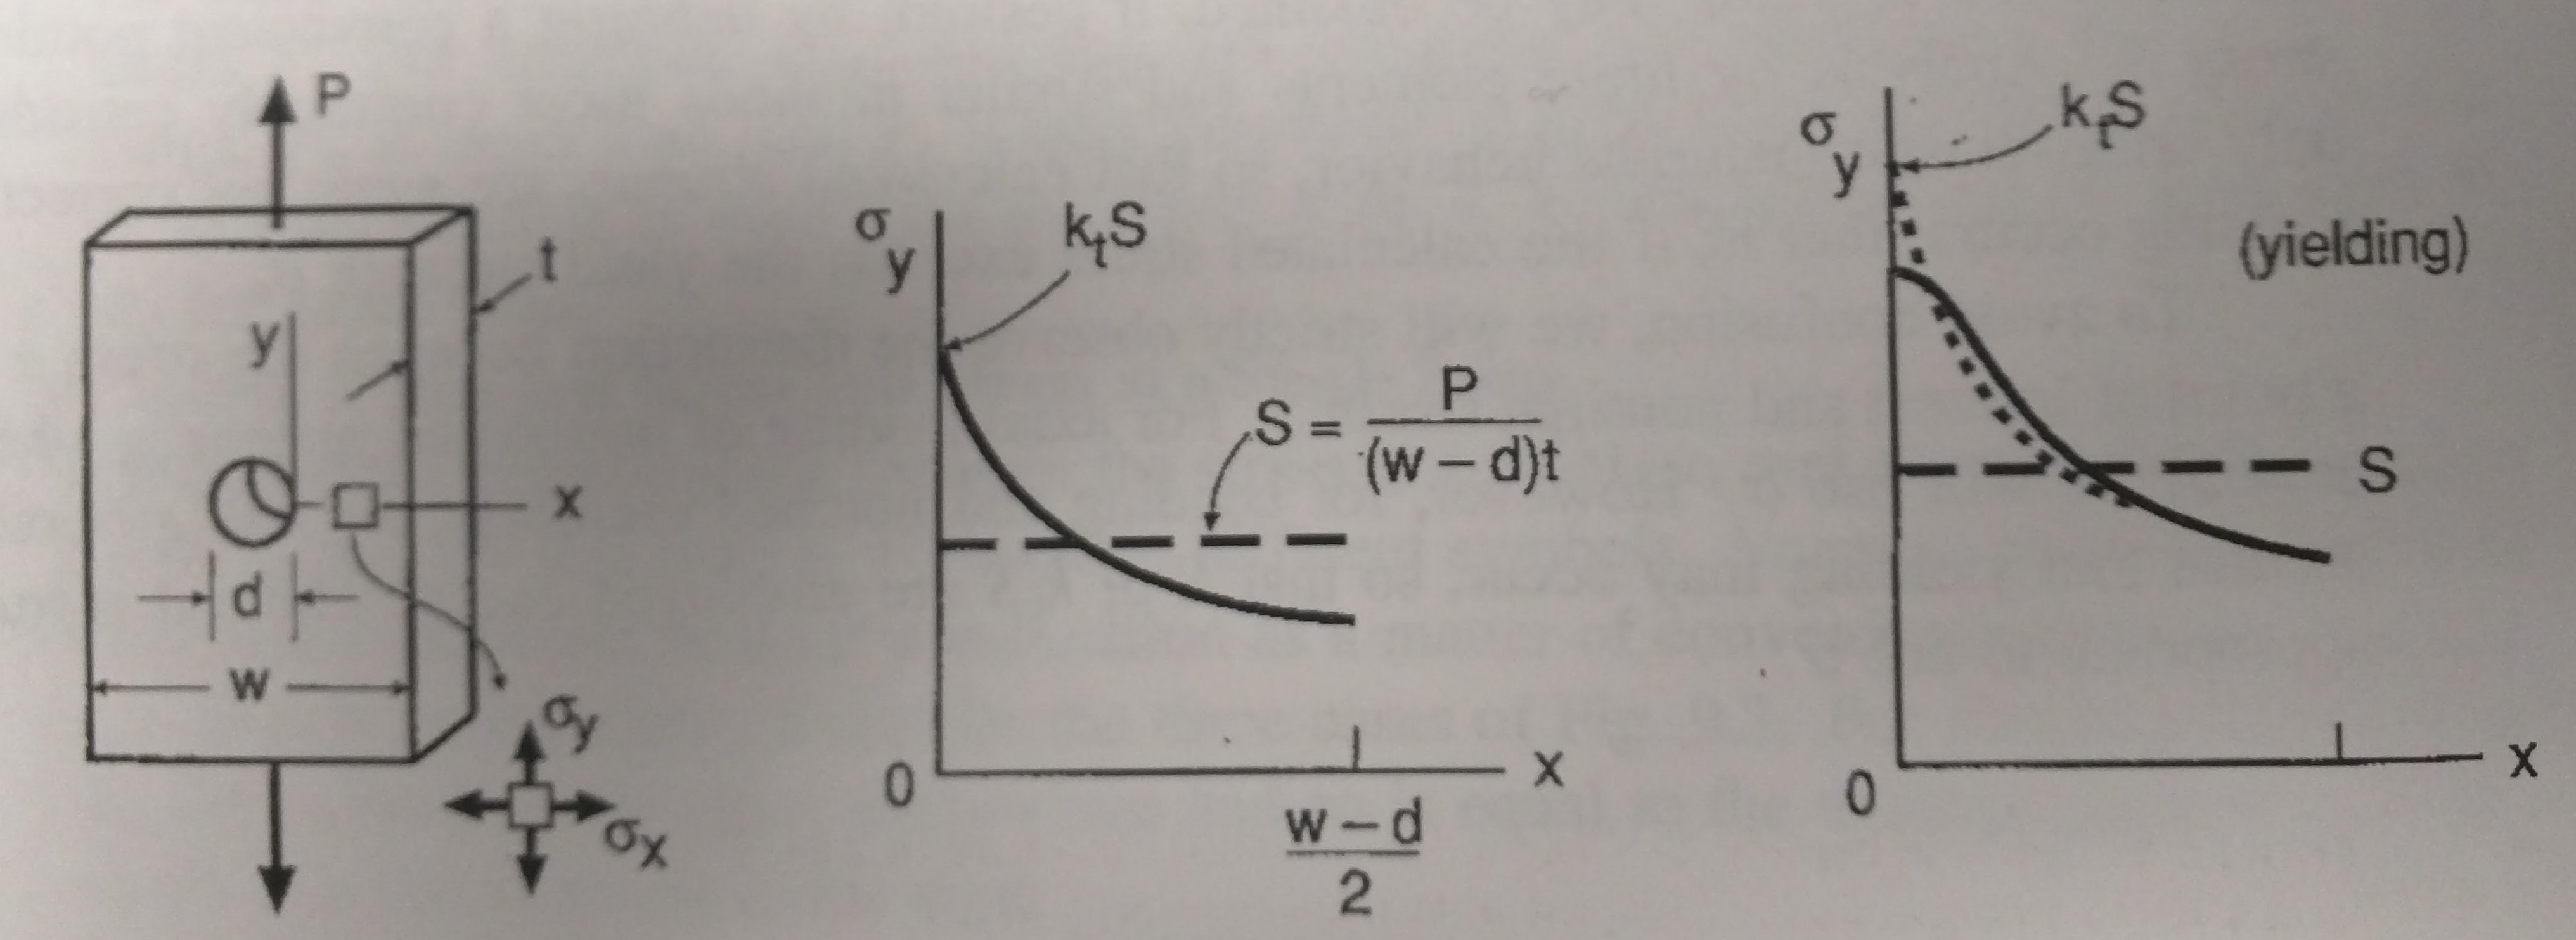
\includegraphics{../images/p232-c.jpg}
\end{frame}

\hypertarget{fatigue-tests}{%
\section{fatigue tests}\label{fatigue-tests}}

\begin{frame}{rotating cantilever beam}
\protect\hypertarget{rotating-cantilever-beam}{}
\begin{figure}
\centering
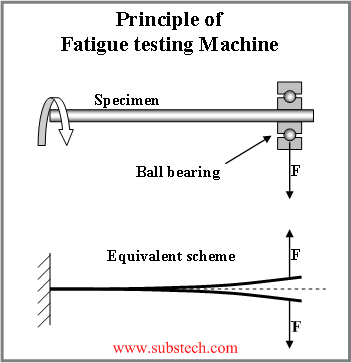
\includegraphics{../images/rotating_cantilever.png}
\caption{Stress variation through a cantilever beam}
\end{figure}
\end{frame}

\begin{frame}{rotating four-point bend}
\protect\hypertarget{rotating-four-point-bend}{}
\begin{figure}
\centering
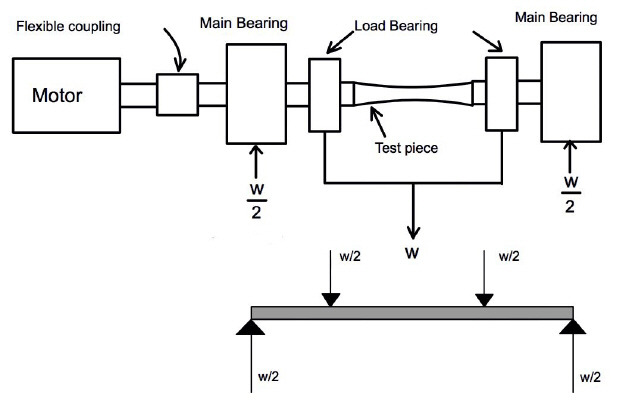
\includegraphics{../images/Rotating_Bending_Machine.jpg}
\caption{Four-point bend test gives uniform stress along the top and
bottom surfaces}
\end{figure}
\end{frame}

\begin{frame}{fatigue tests}
\protect\hypertarget{fatigue-tests-1}{}
\begin{itemize}
\tightlist
\item
  The above rotating methods are very common, but in their current
  configurations can only be used for zero mean stress
\item
  a reciprocating bend test can be used for non-zero mean stress
\end{itemize}
\end{frame}

\begin{frame}{reciprocating bend test}
\protect\hypertarget{reciprocating-bend-test}{}
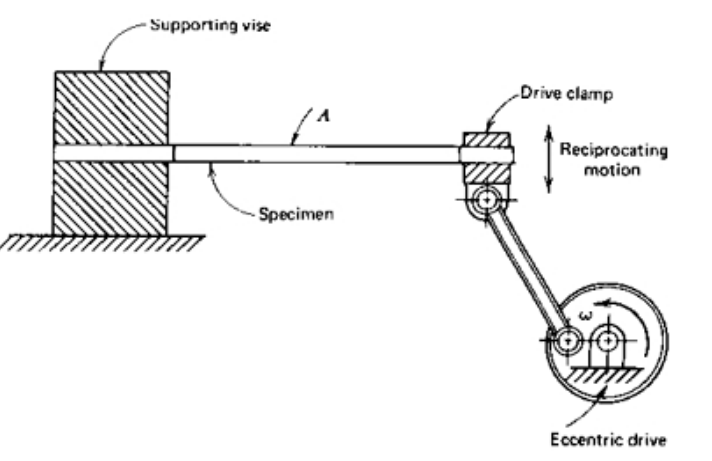
\includegraphics{../images/reciprocating_cantilever.PNG}
\end{frame}

\begin{frame}{axial fatigue test}
\protect\hypertarget{axial-fatigue-test}{}
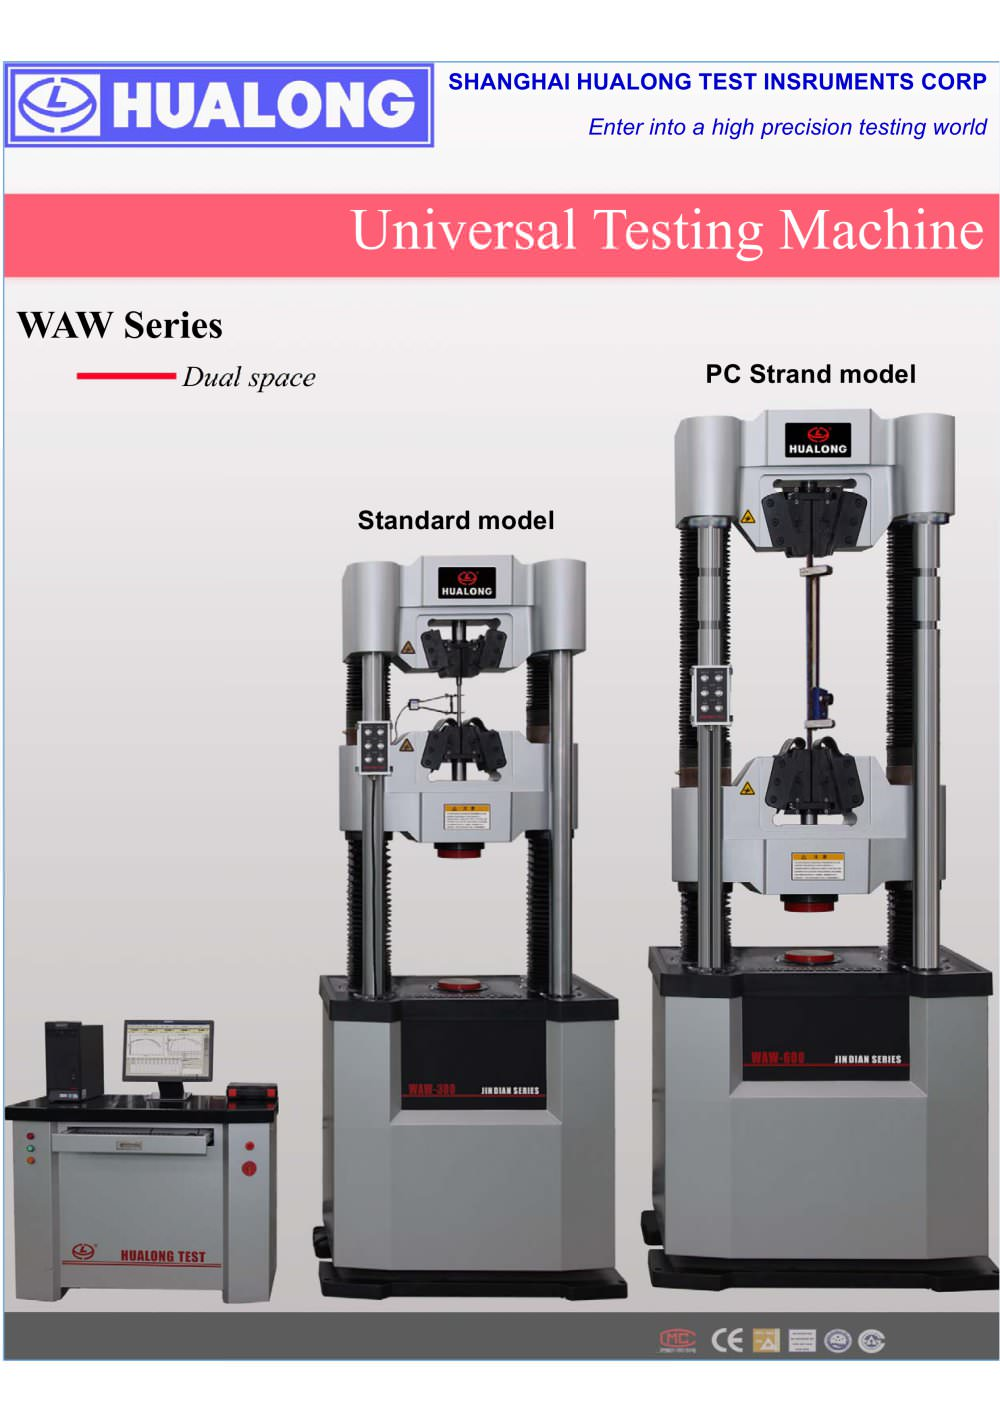
\includegraphics{../images/servohydraulic.jpg}
\end{frame}

\begin{frame}{fatigue tests}
\protect\hypertarget{fatigue-tests-2}{}
\begin{itemize}
\tightlist
\item
  The length of a fatigue test is determined by two factors

  \begin{enumerate}
  \tightlist
  \item
    How many cycles it takes for the specified load to cause failure
  \item
    The speed of the motor controlling the test
  \end{enumerate}
\end{itemize}
\end{frame}

\begin{frame}{fatigue tests}
\protect\hypertarget{fatigue-tests-3}{}
\begin{itemize}
\tightlist
\item
  Servohydraulic machines generally have a speed of 10 - 100 Hz.
\item
  At a speed of 100 Hz, it would take 28 hours for 107 cycles, 12 days
  for 108 cycles, and nearly 4 months for 109 cycles
\item
  While some machines can test at very high speeds, the inertia of the
  sample can interfere with results
\end{itemize}
\end{frame}

\end{document}
